% Magnecko Sense board datasheet. Standalone source: no external assets needed.
% Build with pdfLaTeX (two passes), latexmk -pdf, or Tectonic.
% Edit document metadata here; cross-check hardware identity against
% common/board/board_identity.h and config/flash_parameters.json.
\documentclass[10pt,a4paper]{article}
\usepackage[T1]{fontenc}
\usepackage{iftex}
\ifPDFTeX\usepackage[utf8]{inputenc}\fi
\usepackage{helvet}
\renewcommand{\familydefault}{\sfdefault}
\usepackage[scaled=0.88]{beramono}
\usepackage[a4paper,left=18mm,right=18mm,top=24mm,bottom=21mm,
  headheight=30pt,headsep=7mm,footskip=11mm]{geometry}
\usepackage[table]{xcolor}
\usepackage{microtype}
\usepackage{array,booktabs,tabularx}
\usepackage{enumitem}
\usepackage{titlesec}
\usepackage{fancyhdr,lastpage}
\usepackage{tikz}
\usetikzlibrary{arrows.meta,positioning,calc,fit,backgrounds}
\usepackage{caption}
\usepackage{hyperref}

% Document identity. Hardware revision 0 is a literal trailing hyphen.
\newcommand{\ProductName}{Magnecko Sense}
\newcommand{\BoardVersion}{MGS-1.0-}
\newcommand{\DocumentID}{MGS-DS-001}
\newcommand{\DocumentRevision}{A}
\newcommand{\DocumentDate}{October 2026}
\newcommand{\DocumentStatus}{PRELIMINARY}

% Original Magnecko styling, inspired by semiconductor datasheet conventions.
\definecolor{MGSRed}{HTML}{B71930}
\definecolor{MGSInk}{HTML}{1C2630}
\definecolor{MGSMuted}{HTML}{52616D}
\definecolor{MGSRule}{HTML}{C9D0D5}
\definecolor{MGSGray}{HTML}{F0F3F5}
\definecolor{MGSPale}{HTML}{FBF0F2}
\definecolor{LEDAmber}{HTML}{A56600}
\definecolor{LEDBlue}{HTML}{2869B0}
\definecolor{LEDGreen}{HTML}{20854C}
\definecolor{LEDCyan}{HTML}{087F8C}
\definecolor{LEDMagenta}{HTML}{A12883}
\color{MGSInk}
\hypersetup{colorlinks=true,linkcolor=MGSRed,urlcolor=MGSRed,
  pdftitle={Magnecko Sense -- MGS-1.0- Board Datasheet},
  pdfauthor={Magnecko},pdfsubject={Preliminary hardware and firmware interface reference},
  pdfkeywords={Magnecko Sense, MGS, STM32N657, VL53L9, datasheet},
  bookmarksnumbered=true}
\urlstyle{same}
\setlength{\parindent}{0pt}
\setlength{\parskip}{4pt}
\setlength{\tabcolsep}{6pt}
\renewcommand{\arraystretch}{1.12}
\setlength{\emergencystretch}{1.5em}
\setlist[itemize]{leftmargin=1.25em,itemsep=3pt,topsep=4pt,parsep=0pt,
  before=\raggedright,
  label=\textcolor{MGSRed}{\raisebox{0.15ex}{\scriptsize\textbullet}}}
\setlist[enumerate]{leftmargin=1.6em,itemsep=4pt,topsep=4pt,parsep=0pt}
\titleformat{\section}{\large\bfseries\color{MGSRed}}{\thesection}{0.6em}{}
\titleformat{\subsection}{\normalsize\bfseries}{\thesubsection}{0.6em}{}
\titlespacing*{\section}{0pt}{10pt}{7pt}
\titlespacing*{\subsection}{0pt}{9pt}{4pt}
\captionsetup{font=small,labelfont=bf,justification=centering,skip=5pt,hypcap=false}
\newcolumntype{L}[1]{>{\raggedright\arraybackslash}p{#1}}
\newcolumntype{Y}{>{\raggedright\arraybackslash}X}
\newcommand{\thead}[1]{\textbf{#1}}
\newcommand{\code}[1]{\texttt{\detokenize{#1}}}
\newcommand{\source}[1]{\par\nobreak{\scriptsize\color{MGSMuted}Source: \path{#1}.\par}}
\newcommand{\tabtitle}[1]{\par\smallskip{\small\bfseries #1}\par\smallskip}
\newcommand{\note}[2]{\par\medskip\begingroup
  \setlength{\fboxsep}{9pt}\noindent
  \colorbox{MGSGray}{\parbox{\dimexpr\linewidth-18pt\relax}{
  \small\textbf{\textcolor{MGSRed}{#1}}\enspace #2}}\par\endgroup\medskip}
\newcommand{\led}[2]{\tikz[baseline=-0.6ex]\fill[#1] (0,0) circle (0.8mm);\enspace #2}
\newcommand{\pageintro}[1]{{\small\color{MGSMuted}#1\par}\medskip}

\pagestyle{fancy}
\fancyhf{}
\fancyhead[L]{\textcolor{MGSRed}{\Large\bfseries MGS}\hspace{8pt}
  {\small\bfseries\ProductName}}
\fancyhead[R]{{\small\bfseries\BoardVersion}\\[-1pt]
  {\scriptsize\color{MGSMuted}\DocumentID\; Rev.\ \DocumentRevision\; |\; \DocumentDate}}
\renewcommand{\headrulewidth}{0.6pt}
\renewcommand{\headrule}{\hbox to\headwidth{\color{MGSRed}\leaders\hrule height \headrulewidth\hfill}}
\fancyfoot[L]{\scriptsize\color{MGSMuted}magnecko\quad |\quad \DocumentStatus}
\fancyfoot[C]{\scriptsize\color{MGSMuted}\DocumentID\; Rev.\ \DocumentRevision}
\fancyfoot[R]{\small\bfseries\thepage\, /\, \pageref*{LastPage}}
\renewcommand{\footrulewidth}{0.3pt}

\tikzset{
  block/.style={draw=MGSInk,line width=0.6pt,fill=white,rounded corners=1.5pt,
    align=center,minimum height=12mm,font=\small,inner sep=5pt},
  core/.style={block,draw=MGSRed,fill=MGSPale,line width=0.9pt},
  bus/.style={-{Stealth[length=2mm]},line width=0.7pt,draw=MGSInk},
  twoway/.style={{Stealth[length=1.7mm]}-{Stealth[length=1.7mm]},line width=0.7pt},
  buslabel/.style={font=\scriptsize,fill=white,inner sep=2pt,text=MGSMuted}}

\begin{document}

% --------------------------------------------------------------------------
% PAGE 1 -- product overview, two-column opening, vector block diagram.
% --------------------------------------------------------------------------
{\color{MGSRed}\small\bfseries MULTIZONE DEPTH + INERTIAL SENSING}\par
\vspace{2mm}
{\fontsize{28}{31}\selectfont\bfseries\ProductName}\par
\vspace{1mm}
{\fontsize{14}{18}\selectfont Multizone time-of-flight and six-axis IMU board\\
with USB and Ethernet streaming}\par
\vspace{4mm}

\begin{minipage}[t]{0.475\linewidth}
\vspace{0pt}
\section{Features}\label{sec:features}
\begin{itemize}
  \item VL53L9 multizone time-of-flight acquisition; up to
    \textbf{54 $\times$ 42 depth zones} in the current interface.
  \item LSM6DSV16X acceleration, angular rate, and SFLP game-rotation quaternion.
  \item STM32N657 processing with ThreadX, USBX, and NetX Duo.
  \item USB CDC ACM and Ethernet TCP streaming; both interfaces can operate together.
  \item Runtime ranging control: start, stop, reset, configuration, and sensor shutdown.
  \item 64\,MiB external NOR flash; A/B application slots with verified trial boot and fallback.
  \item Autonomous RGB status patterns for boot, initialization, ranging, idle, and faults.
  \item Device identity, image provenance, and CPU profiling telemetry.
\end{itemize}
\section{Applications}\label{sec:applications}
\begin{itemize}
  \item Depth-sensing and motion-estimation prototypes
  \item Robotics perception and interaction experiments
  \item Sensor evaluation, recording, and reconstruction
\end{itemize}
\end{minipage}\hfill
\begin{minipage}[t]{0.475\linewidth}
\vspace{0pt}
\section{Description}\label{sec:description}
\ProductName\ combines a multizone depth sensor and six-axis inertial sensor
with an STM32N657 controller. The firmware acquires depth over MIPI CSI-2,
controls the ToF device over I3C, and publishes depth and inertial packets to a
host over USB or Ethernet.

The common host framing carries sensor data, acknowledged control commands,
device parameters, and diagnostic information. The Device Monitor provides
live visualization and sensor controls. An independent update service programs
the inactive application slot and supports trial-boot confirmation and fallback.

\tabtitle{Board identification}
{\small
\begin{tabularx}{\linewidth}{@{}L{0.38\linewidth}Y@{}}
\toprule
\rowcolor{MGSGray}\thead{Item} & \thead{Value} \\
\midrule
Product & \ProductName \\
PCB identifier & MGS \\
Hardware baseline & \BoardVersion \\
Firmware repository & \code{magnecko-sense-fw} \\
Document status & Preliminary engineering data \\
\bottomrule
\end{tabularx}}
\vspace{2mm}
{\small\color{MGSMuted}This document describes the current firmware implementation.
Electrical, optical, thermal, and mechanical board ratings await characterization;
software settings are not measured performance guarantees.}
\end{minipage}

\vspace{5mm}
\begin{center}
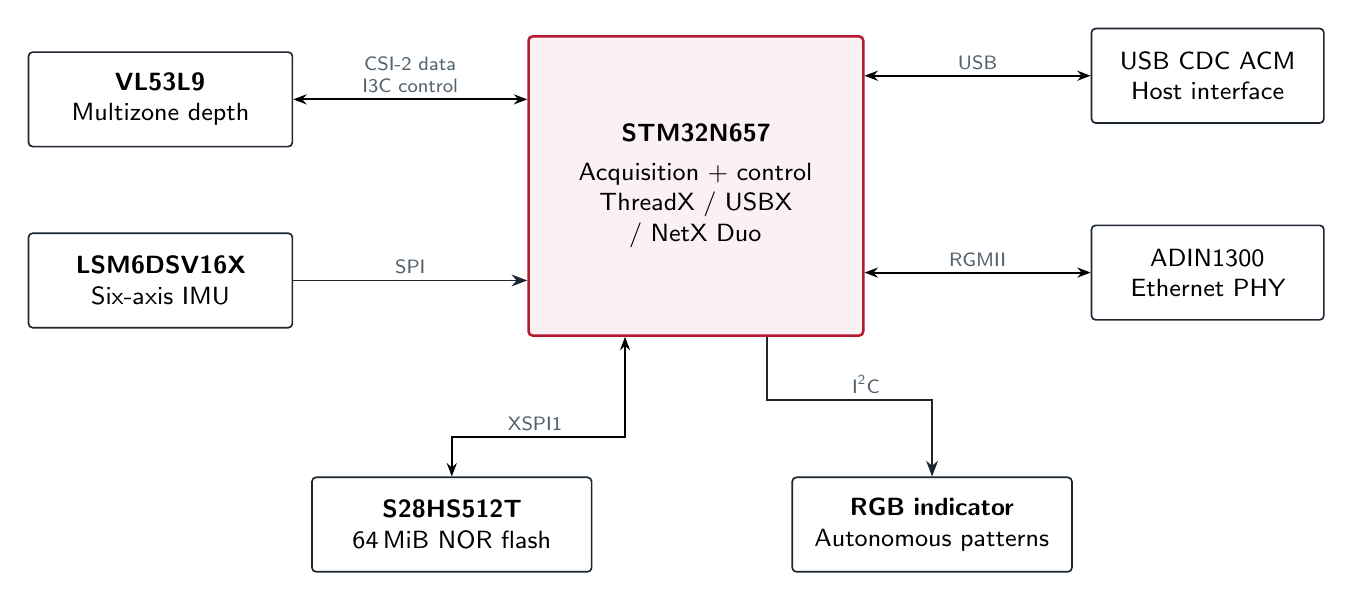
\begin{tikzpicture}[x=1mm,y=1mm]
  \node[block,text width=30mm] (tof) at (20,30) {\textbf{VL53L9}\\Multizone depth};
  \node[block,text width=30mm] (imu) at (20,7) {\textbf{LSM6DSV16X}\\Six-axis IMU};
  \node[core,text width=39mm,minimum height=38mm] (mcu) at (88,19)
    {\textbf{STM32N657}\\[3pt]Acquisition + control\\ThreadX / USBX / NetX Duo};
  \node[block,text width=26mm] (usb) at (153,33) {USB CDC ACM\\Host interface};
  \node[block,text width=26mm] (eth) at (153,8) {ADIN1300\\Ethernet PHY};
  \node[block,text width=32mm] (flash) at (57,-24) {\textbf{S28HS512T}\\64\,MiB NOR flash};
  \node[block,text width=32mm] (led) at (118,-24) {\textbf{RGB indicator}\\Autonomous patterns};
  \draw[twoway] (tof.east) -- node[buslabel,above,align=center] {CSI-2 data\\I3C control} (mcu.west |- tof.east);
  \draw[bus] (imu.east) -- node[buslabel,above] {SPI} (mcu.west |- imu.east);
  \draw[twoway] (mcu.east |- usb.west) -- node[buslabel,above] {USB} (usb.west);
  \draw[twoway] (mcu.east |- eth.west) -- node[buslabel,above] {RGMII} (eth.west);
  \draw[twoway] (flash.north) -- ++(0,5) -| node[buslabel,pos=0.24,above] {XSPI1} ([xshift=-9mm]mcu.south);
  \draw[bus] ([xshift=9mm]mcu.south) -- ++(0,-8) -| node[buslabel,pos=0.3,above] {I\textsuperscript{2}C} (led.north);
\end{tikzpicture}
\captionof{figure}{Simplified functional block diagram. Connections represent logical interfaces.}
\end{center}

\newpage
% --------------------------------------------------------------------------
% PAGE 2 -- specifications, with software limits distinguished from ratings.
% --------------------------------------------------------------------------
\section{Specifications}\label{sec:specifications}
\pageintro{Configuration reference for \BoardVersion. Values below describe the
current implementation unless explicitly identified otherwise.}

\subsection{Hardware and firmware resources}
{\small\begin{tabularx}{\linewidth}{@{}L{36mm}L{40mm}Y@{}}
\toprule
\rowcolor{MGSGray}\thead{Function} & \thead{Device / allocation} & \thead{Implemented role} \\
\midrule
Main controller & STM32N657 & Acquisition, control, transports, and image boot \\
Depth sensing & VL53L9 & I3C configuration and CSI-2 RAW8 capture \\
Inertial sensing & LSM6DSV16X & Acceleration, gyroscope, and SFLP game quaternion \\
Ethernet PHY & ADIN1300 & RGMII host link with link-state recovery \\
External NOR & S28HS512T; 64\,MiB & Parameters, FSBL, application slots, update records \\
Application image & 512\,KiB maximum & SRAM-loaded image, including header and padding \\
Device parameters & 16\,KiB reader limit & UTF-8 JSON identity and build metadata \\
\bottomrule
\end{tabularx}}

\subsection{Firmware configuration limits}
{\small\begin{tabularx}{\linewidth}{@{}Y L{33mm}L{47mm}@{}}
\toprule
\rowcolor{MGSGray}\thead{Parameter} & \thead{Setting / range} & \thead{Conditions} \\
\midrule
ToF frame period & 10--1000\,ms & Host control validation range \\
ToF exposure & 1--30\,ms & Integer; exposure $\leq$ frame period \\
ToF binning & 2, 4, 6, 8, 12, 24 & Geometry changes with binning \\
ToF power mode & Regular / low / ultra low & Subject to sensor acceptance \\
Range context & Short / long & DSS required in long context \\
IMU acceleration full scale & $\pm4\,g$ & Current initialization setting \\
IMU angular-rate full scale & $\pm1000\,^{\circ}\!$/s & Current initialization setting \\
IMU / SFLP update rate & 120\,Hz & Device acquisition configuration \\
IMU packet publication & 100\,Hz target & Host delivery subject to backpressure \\
\bottomrule
\end{tabularx}}
{\footnotesize\color{MGSMuted}Passing host validation does not guarantee sensor
acceptance of every combination. Query the acknowledged configuration and measure
delivered frame rate for the selected exposure, mode, and transport.}

\subsection{Depth geometry}
{\small\begin{tabularx}{\linewidth}{@{}L{20mm}Y Y Y r@{}}
\toprule
\rowcolor{MGSGray}\thead{Binning} & \thead{Raw zones} & \thead{Default crop} & \thead{CSI bytes $\times$ rows} & \thead{Payload (B)} \\
\midrule
2  & $54\times42$ & $54\times42$ & $100\times149$ & 14\,900 \\
4  & $24\times24$ & $24\times20$ & $100\times39$  & 3\,900 \\
6  & $18\times14$ & $18\times14$ & $100\times18$  & 1\,800 \\
8  & $12\times10$ & $12\times10$ & $100\times9$   & 900 \\
12 & $8\times8$   & $8\times6$   & $100\times6$   & 600 \\
24 & $4\times4$   & $4\times4$   & $100\times3$   & 300 \\
\bottomrule
\end{tabularx}}
{\footnotesize CSI dimensions describe transported bytes, not depth-zone count.
Decode crop and DSS layout from the final 100-byte sensor metadata row.}

\subsection{Board characterization status}
{\small\begin{tabularx}{\linewidth}{@{}L{55mm}Y@{}}
\toprule
\rowcolor{MGSGray}\thead{Board specification} & \thead{Status} \\
\midrule
Input ratings / consumption & Board-level electrical limits and absolute ratings not established \\
Optical performance & Range, accuracy, FoV, and latency characterization pending \\
Temperature / thermal limits & Board-level characterization pending \\
Mechanical / connector definition & Released outline, mounting, and pinout drawings not supplied \\
\bottomrule
\end{tabularx}}
\source{Appli/Libs/53L9/interface/vl53l9/vl53l9_utils.c}
\source{Appli/Libs/control/tof_control.c; Appli/Libs/IMU/IMU.c}

\newpage
% --------------------------------------------------------------------------
% Host interface information.
% --------------------------------------------------------------------------
\section{Host interfaces and data format}\label{sec:interfaces}
\pageintro{USB and Ethernet share the same sensor framing and control semantics.
Connection endpoints below are the current firmware defaults.}

\subsection{Interface summary}
{\small\begin{tabularx}{\linewidth}{@{}L{30mm}L{46mm}Y@{}}
\toprule
\rowcolor{MGSGray}\thead{Interface} & \thead{Endpoint} & \thead{Behavior} \\
\midrule
USB & CDC ACM; assert DTR & One serial owner. Host baud-rate selection does not determine USB throughput. \\
Ethernet streaming & \code{192.168.8.20:50002} & One TCP stream client; telemetry and sensor commands \\
Ethernet update & TCP port 50003 & Application update and persistent update status \\
Legacy service & TCP port 50000 & Echo only; not the sensor command endpoint \\
Debug / provisioning & SWD / ST-Link & SRAM development and initial flash programming; use the board boot configuration appropriate to debug access. \\
\bottomrule
\end{tabularx}}

USB and Ethernet can be active simultaneously. An Ethernet disconnect invalidates
the old TCP session; reconnect and clear partial receive buffers. USB and sensor
operation continue independently of Ethernet link recovery.

\subsection{Common packet header}
All multi-byte integers are little-endian. The 16-byte header is followed
immediately by the specified payload; packets have no inter-packet padding.

{\small\begin{tabularx}{\linewidth}{@{}L{22mm}L{21mm}L{35mm}Y@{}}
\toprule
\rowcolor{MGSGray}\thead{Byte offset} & \thead{Size} & \thead{Field} & \thead{Meaning} \\
\midrule
0 & 4 bytes & Magic & Packet type, encoded as ASCII \\
4 & 4 bytes & Sequence / request ID & Independent sensor counter or command correlation \\
8 & 4 bytes & Payload length & Bytes following the common header \\
12 & 2 bytes & Field A & Type-specific version, width, or channel count \\
14 & 2 bytes & Field B & Type-specific operation, height, or version \\
\bottomrule
\end{tabularx}}

\subsection{Packet types and measurement units}
{\small\begin{tabularx}{\linewidth}{@{}L{18mm}L{32mm}Y@{}}
\toprule
\rowcolor{MGSGray}\thead{Magic} & \thead{Payload size} & \thead{Content} \\
\midrule
\code{VL9F} & Up to 14\,900 bytes & CSI frame: radial distance, amplitude, ambient, optional DSS, padding, and metadata \\
\code{IMUF} & 44 bytes & Millisecond timestamp; acceleration in mg; gyro in mdps; quaternion X/Y/Z/W as binary32 \\
\code{TOFS} & 36 bytes (v2) & Sensor state, command result, configuration, geometry, and frame counter \\
\code{PARM} & Up to 16\,384 bytes & UTF-8 JSON device identity and stored build provenance \\
\code{PROF} & $44+48N$ bytes & CPU interval and $N$ thread records ($0\leq N\leq64$) \\
\code{CTRL} & 0 or 12 bytes & Host-to-board sensor command and optional settings \\
\bottomrule
\end{tabularx}}

\subsection{Depth interpretation and stream handling}
Depth words use bits 0--14 for raw radial distance in millimetres. Bit 15 selects
the ranging step; it is not an invalid-data flag. The monitor treats zero distance
as a missing return. Raw values are not calibrated, confidence-filtered,
perpendicular-depth measurements. The IMU game quaternion has no compass-heading
reference.

TCP and USB reads may split or combine packets. Buffer complete frames, validate
lengths, and consume exactly header plus payload. A slow client can lose depth
or IMU samples; use sequence counters to detect gaps. The common sensor header
does not provide a payload CRC.
\source{wiki/protocols/wire-protocol.md}

\newpage
% --------------------------------------------------------------------------
% Boot flow and memory map.
% --------------------------------------------------------------------------
\section{Boot, storage, and firmware updates}\label{sec:boot}
\pageintro{Persistent applications execute from SRAM after selection and validation
by the first-stage bootloader. Flash slot capacity and execution capacity differ.}

\subsection{Boot sequence}
\begin{center}
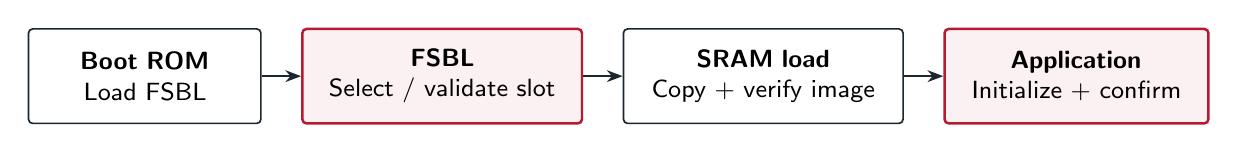
\begin{tikzpicture}[node distance=5mm]
  \node[block,text width=26mm] (rom) {\textbf{Boot ROM}\\Load FSBL};
  \node[core,text width=32mm,right=of rom] (select) {\textbf{FSBL}\\Select / validate slot};
  \node[block,text width=32mm,right=of select] (copy) {\textbf{SRAM load}\\Copy + verify image};
  \node[core,text width=30mm,right=of copy] (app) {\textbf{Application}\\Initialize + confirm};
  \draw[bus] (rom) -- (select);
  \draw[bus] (select) -- (copy);
  \draw[bus] (copy) -- (app);
\end{tikzpicture}
\captionof{figure}{Normal boot path. A failed trial can fall back to the confirmed application.}
\end{center}
The application image is copied to \code{0x34000000}; its vector table is at
\code{0x34000400}. The current signed image limit is 512\,KiB, including the STM32
v2.3 header and alignment padding. The persistent boot path and direct SRAM
development path exercise different initialization conditions.

\subsection{External NOR allocation}
The 64\,MiB device is accessed through XSPI1 and XSPIM port 2. Its memory-mapped
window starts at \code{0x90000000} and ends before \code{0x94000000}.

{\small\begin{tabularx}{\linewidth}{@{}Y L{30mm}L{30mm}r@{}}
\toprule
\rowcolor{MGSGray}\thead{Region} & \thead{Flash offset} & \thead{CPU address} & \thead{Reserved} \\
\midrule
Parameter JSON & \code{0x00000000} & \code{0x90000000} & 256\,KiB \\
FSBL2 & \code{0x00040000} & \code{0x90040000} & 512\,KiB \\
Reserved & \code{0x000C0000} & \code{0x900C0000} & 256\,KiB \\
Application A & \code{0x00100000} & \code{0x90100000} & 8\,MiB \\
Application B & \code{0x00900000} & \code{0x90900000} & 8\,MiB \\
Update metadata A & \code{0x01100000} & \code{0x91100000} & 256\,KiB \\
Update metadata B & \code{0x01140000} & \code{0x91140000} & 256\,KiB \\
Future data & \code{0x01180000} & \code{0x91180000} & 46.5\,MiB \\
\bottomrule
\end{tabularx}}

\subsection{Update and recovery behavior}
An application update writes the inactive slot and verifies the transferred
image before committing pending-boot metadata. Alternating metadata sectors
retain confirmed and pending image descriptors, hashes, and trial state. Trial
boot confirmation and the watchdog allow fallback to the confirmed application.

USB CDC and TCP port 50003 support updates. A transfer has one owning session;
an incomplete upload is aborted after disconnect or timeout. Uploads restart
from the beginning. Inspect update status after an interrupted or uncertain
operation before starting a new transfer.

\note{Image validation}{SHA-256, checksums, and structural validation detect
corruption. The current packaging flow uses the STM32 signing tool with no key;
this document does not claim cryptographic publisher authentication.}

\subsection{Parameters and production identity}
The first 256\,KiB holds compact UTF-8 JSON, a NUL terminator, and erased padding.
The application reads at most 16\,KiB at startup and reports the cached object
through \code{PARM}. Ordinary programming preserves existing per-device identity
and calibration. An explicit settings replacement is required to relabel an
already programmed board. Application DFU does not rewrite this parameter JSON.
\source{common/firmware/fw_update.h; scripts/build.sh}
\source{wiki/hardware/flash-layout.md; wiki/firmware/firmware-updates.md}

\newpage
% --------------------------------------------------------------------------
% Operational states and diagnostic LED legend.
% --------------------------------------------------------------------------
\section{Operating states and indicators}\label{sec:states}
\pageintro{The RGB indicator follows boot progress and the acknowledged ToF state.
Patterns are generated autonomously by the LED controller.}

{\small\begin{tabularx}{\linewidth}{@{}L{35mm}L{48mm}Y@{}}
\toprule
\rowcolor{MGSGray}\thead{State} & \thead{Indication} & \thead{Meaning} \\
\midrule
FSBL started & \led{LEDAmber}{Amber blink, about 2\,Hz} & GPIO and I\textsuperscript{2}C configured; flash initialization follows. \\
FSBL loading & \led{LEDAmber}{Amber blink, about 5\,Hz} & Reading metadata, selecting a slot, and loading the image. \\
FSBL handoff & \led{LEDMagenta}{Solid magenta} & SRAM copy verified; application branch is being prepared. \\
FSBL error & \led{LEDAmber}{Counted amber burst + 2\,s gap} & Bootloader error; flash / metadata / image stage encoded by the count. \\
Application started & \led{LEDBlue}{Blue blink, about 2\,Hz} & Application GPIO and I\textsuperscript{2}C are configured. \\
Core init finished & \led{LEDCyan}{Cyan double pulse + pause} & RTOS / middleware setup finished; sensor setup may continue. \\
ToF ranging & \led{LEDGreen}{Green breathing, about 1.2\,s} & Sensor successfully entered ranging state. \\
ToF idle & \led{LEDBlue}{Dim blue breathing, about 2.4\,s} & Ranging stopped, including after a successful sensor reset. \\
ToF powered down & \led{LEDAmber}{Dim steady amber} & XSHUT asserted; sensor supply rails remain connected. \\
ToF resetting & \led{LEDCyan}{Cyan blink, about 5\,Hz} & Sensor reinitialization is in progress. \\
ToF fault & \led{MGSRed}{Red double pulse + pause} & Latched sensor, capture, or initialization fault. \\
Fatal application error & Counted red / blue / magenta burst & Fatal startup stage encoded by color and count; 2\,s dark between bursts. \\
\bottomrule
\end{tabularx}}

\subsection{Sensor control sequence}
Ranging starts at boot using the compiled profile. To change settings, send
\code{STOP}, wait for its successful \code{TOFS} acknowledgement, send
\code{SET_CONFIG}, wait for success, then send \code{START}. Settings and
start/stop state are volatile; a board reset restores the compiled profile.

\code{RESET} affects the ToF sensor only. It restores compiled defaults and
leaves ranging stopped; issue \code{START} separately. \code{POWER_DOWN} stops
capture and asserts XSHUT. Recover with \code{RESET}, followed by \code{START}.
Idle and sensor power-down do not stop the IMU, USB, or networking.

Faults remain latched until an explicit sensor reset or board reset. Commands
return a state snapshot; rejected commands leave the acknowledged state intact.
Allow one outstanding sensor command per connection and match both its request
ID and operation before continuing.

\subsection{Reading boot progress}
Startup patterns can be brief; no artificial display delays are inserted.
Fault bursts use 200\,ms on / off pulses and a 2\,s gap; the full code table is
in the status-LED guide. Earlier double-pulse encodings could appear continuous.
Persistent magenta narrows investigation to the handoff or early application
startup, but does not prove that application code has executed. No indication
can also mean failure before LED setup or an unavailable LED device.

Because the LED engine runs independently, the last pattern may survive a CPU
hang. Treat it as the last reported state, rather than a continuous processor
heartbeat. Green indicates ranging was started; it does not establish delivered
frame rate or the presence of a host connection.
\source{wiki/firmware/status-led.md; common/led/LEDController.c}

\newpage
% --------------------------------------------------------------------------
% Application guidance, version standard, and maintainable references.
% --------------------------------------------------------------------------
\section{Application information}\label{sec:integration}
\pageintro{Use the repository wiki for complete build, programming, and byte-level
protocol instructions. This section provides the integration sequence.}

\subsection{Host integration sequence}
\begin{enumerate}
  \item Confirm PCB / assembly identity and supply arrangement; complete the
    board bring-up checks before characterization.
  \item Provision FSBL, the baseline application, and device parameters with the
    external loader. Use Release firmware for normal operation.
  \item Connect USB CDC with DTR asserted, or TCP port 50002 with the host at a
    different address on \code{192.168.8.0/24}.
  \item Read \code{PARM} and \code{GET_CONFIG}; record firmware provenance,
    hardware identity, and acknowledged sensor settings.
  \item Decode complete frames and metadata crop; monitor sequence gaps and
    \code{TOFS} errors. Measure delivered rate and latency for the actual setup.
\end{enumerate}

\subsection{Power and mechanical integration}
USB PD sink profiles in firmware are not board input ratings. Dead-battery
startup on \BoardVersion\ requires hardware validation. Establish input
conditions, consumption, startup, and thermal performance on the actual assembly.

Dimensions, mounting, optical keep-out, connector numbering, and orientation
require released PCB / mechanical drawings. Figure~1 shows logical interfaces,
not physical connector assignments or scale.

\section{Identification and document support}\label{sec:support}
\subsection{Hardware version standard}
Use \code{MGS-<MAJOR>.<MINOR><REVISION>}. Revision 0 is a literal \code{-}; the
next revisions are A, B, and so on. Reset the revision to \code{-} after a major
or minor increment. Never reuse an assigned identifier.

{\small\begin{tabularx}{\linewidth}{@{}L{30mm}Y L{34mm}@{}}
\toprule
\rowcolor{MGSGray}\thead{Change} & \thead{Classification} & \thead{Example result} \\
\midrule
Revision & Correct / refine intended functionality; document workarounds. & \code{MGS-1.0A} \\
Minor & Add functionality while preserving established interfaces. & \code{MGS-1.1-} \\
Major & Introduce incompatible interfaces or architecture. & \code{MGS-2.0-} \\
\bottomrule
\end{tabularx}}

Assembly variants and BOM substitutions on an unchanged layout are tracked
separately. A companion IC that fixes already intended USB PD dead-battery
behavior without changing firmware or external functionality is a revision
change. Record actual capabilities and quirks by revision and assembly variant.

\subsection{Source documents}
{\small\begin{tabularx}{\linewidth}{@{}L{45mm}Y@{}}
\toprule
\rowcolor{MGSGray}\thead{Reference} & \thead{Repository location} \\
\midrule
Build, flash, and debug & \path{wiki/getting-started/build-flash-debug.md} \\
Host wire protocol & \path{wiki/protocols/wire-protocol.md} \\
Boot / update policy & \path{wiki/firmware/firmware-updates.md} \\
Identity and parameter fields & \path{wiki/firmware/parameters.md} \\
Board acceptance test plan & \path{wiki/hardware/bring-up-and-testing.md} \\
\bottomrule
\end{tabularx}}

\subsection{Document revision history}
{\small\begin{tabularx}{\linewidth}{@{}L{16mm}L{32mm}Y@{}}
\toprule
\rowcolor{MGSGray}\thead{Revision} & \thead{Date} & \thead{Change} \\
\midrule
\DocumentRevision & \DocumentDate & Preliminary datasheet for \BoardVersion;
firmware interfaces, counted boot diagnostics, and hardware revision standard. \\
\bottomrule
\end{tabularx}}

\end{document}
